\chapter{A5}

{\LARGE 'Aggregate the two flows representing the same TCP connection; count the total number of TCP connections collected, and the total number of TCP connections that started and finished correctly.'}

\section{Explicação do código desenvolvido}

Este código foi sem dúvida alguma o mais complicado da parte "mandataria". Foi complicado não só codificar mas também perceber o pedido para poder começar a construí-lo. Usámos a mesma estratégia para obter os dados usada previamente. Feito isso precisámos de garantir que o que quer que fizéssemos fosse apenas sobre uma única conexão TCP, daí o \textit{if} que verifica se duas linhas correspondem a mesma conexão. Aí precisámos de saber se a conexão tinha começado e acabado com sucesso. Para fazer isso tivemos que usar as \textit{flags} e concluímos que uma conexão iniciada com sucesso necessita das \textit{flags} \textit{ACK} e \textit{SYN}, e uma conexão terminada com sucesso necessita da \textit{flag} \textit{F}.

\begin{figure}[h!]
    \label{high}
    \centering
    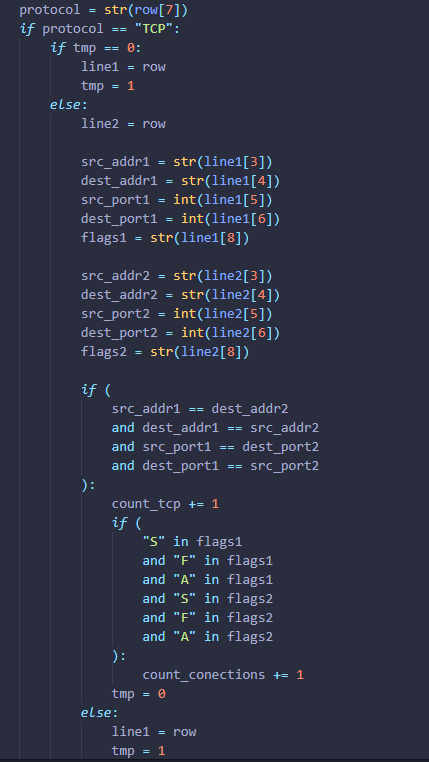
\includegraphics[width=0.8\textwidth]{Images/a5/a5.png}
    \caption{\textit{Código do tópico a5}}
\end{figure}

%----------------------------------------------------------------------------
%----------------------------------------------------------------------------
\clearpage

\section{Resulados obtidos pelo ficheiro www.fct.unl.pt.csv}

Como se pode ver na figura 6.2, foram processadas as linhas do ficheiro www.fct.unl.pt.csv. Apresentamos no output o total de conexões TCP e quantos dessas começaram e terminaram com sucesso.

\begin{figure}[h]
    \label{high}
    \centering
    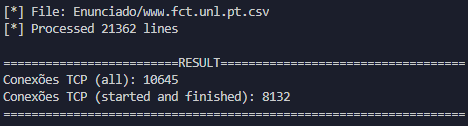
\includegraphics[width=1\textwidth]{Images/a5/a5_a.png}
    \caption{\textit{Output do script a5.py}}
\end{figure}

%----------------------------------------------------------------------------

\section{Resulados obtidos pelo ficheiro bigFlows.csv}

Como se pode ver na figura 6.3, foram processadas as linhas do ficheiro bigFlows.csv. Apresentamos no output o total de conexões TCP e quantos dessas começaram e terminaram com sucesso.

\begin{figure}[h!]
    \label{high}
    \centering
    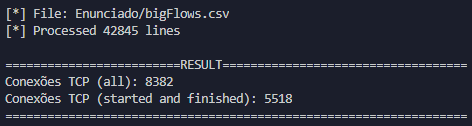
\includegraphics[width=1\textwidth]{Images/a5/a5_b.png}
    \caption{\textit{Output do script a5.py}}
\end{figure}

%----------------------------------------------------------------------------

\clearpage

\section{'Explain the several possible technical reasons that justify why there are TCP connections that were not started or ended correctly.'}

Problemas no inicio das conexões, SYN+ACK.
A conexão está a ser largada em algum sitio durante o envio, geralmente por sistemas intermédios como a \textit{firewall} ou o \textit{load-balancer}. 
Também pode ser algo tão simples como um problema de \textit{routing}.

Problemas no fim da conexões, FIN.
Terminações anormais de conexões podem dever-se a:
\begin{itemize}
    \item Falta de recursos ou interrupção de \textit{internet}.
    \item Uma quebra ou um \textit{bug} na sessão.
    \item Quando um lado da conexão já terminou e fechou a mesma, mas o outro lado continua a enviar dados.
    \item O servidor recusa-se a abrir conexões com o cliente.
\end{itemize}